% Charlotte Geiger - Manuel Lippert - Leonard Schatt
% Physikalisches Praktikum

% 2.Kapitel Fragen zur Vorbereitung

\chapter{Fragen zur Vorbereitung}
\label{chap:fvz}

% Text

% Input der Teilaufgaben je nach Produktion der Nebendateien ohne Ordner
% Charlotte Geiger - Manuel Lippert - Leonard Schatt
% Physikalisches Praktikum

% Teilaufgabe X

\section{Teilaufgabe 1}

\begin{figure}[h]
    \begin{center}
        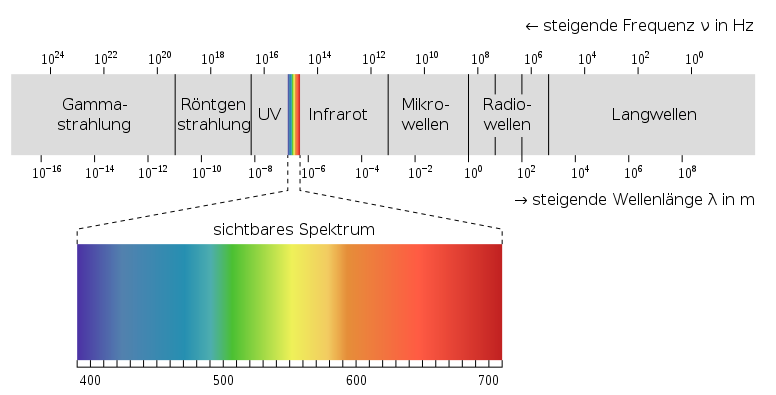
\includegraphics[width=12cm]{Bilder/emspekt.PNG}
    \end{center}
    \caption{Elekromagnetisches Spektrum}
    %\label{fig:meine-grafik}
   \end{figure}
\begin{itemize}
    \item Gammastrahlug: Gammastrahlug entsteht bei einem radioaktiven Gammazerfall. Man setzt sie
    im medizinischen Bereich ein, beispielsweise in der Strahlungstheraphie. Die hochenergetische Strahlung zerstört wucherndes Krebsgewebe indem es die entsprechende DNA zerstört. Sie
    kann nachgewiesen werden in einer Nebenkammer oder einem Geiger-Müller-Zählrohr.
    \item Röntgenstrahlung: Sie wird im medizinischen Bereich verwendet. Außerdem kann man es zur Untersuchung von Strukturen und zur Materialprüfung verwenden. Nachgewiesen kann die Strahlung 
    in Wechselwirkung mit Materie nachgewiesen werden. Man kann beispielsweise Fotoplatten einsetzen. Die Strahlung entsteht durch das Abbremsen von sehr schnellen Elektronen.
    \item UV: Die Strahlung kann sowohl natürlich als auch technisch entstehen. Lampen die UV-Strahlung erzeugen sind beipeilsweise Quecksilberdampf- und Quarzlampen. In diesen Lampen
    entsteht das Licht durch Anregung der jeweiligen Atomen in gasförmiger Phase durch Elektronen. Beim Zurückkehren in den Grundzustand emmittiern sie UV-Strahlung. Man kann die Strahlung
    detektieren, indem man den Photoeffekt nutzt. UV wird umfangreich in der Wirtschaft eingesetzt, unter anderem zur Materialprüfung oder zum aushärten von Polymeren.
    \item Sichtbares Spektrum: Der überwiegende Teil des auf der Erde vorkommenden Lichtes ensteht natürlichvorallem in der Sonne. Man kann es mit Fotoplatten detektieren.
    \item Infrarot: Es existieren Dioden, welche im Infrarotbereich abstrahlen. Man verwendet sie sehr oft bei Fernebedienungen. Infrar kann man mit thermischen Detektoren nachweisen.
    \item Mikrowellen: Mikrowellen entstehen in Laufzeitröhren oder Magnetrons. Die bekannteste technische Anwendung ist die Mikrowelle. Detektieren kann man sie mit einem Mikrowellenmessgerät.
    \item Radiowellen: Diese enstehen auf Radiosendemasten. Dort werden sie von Dipolenantennen erzeugt. Detektieren kann man sie mit einer passenden Antenne und einem Spannungsmessgerät.
    \item Langwellen: Auch diese können in der Natur vorkommen. Detektieren kann man sie mit einer passenden Antenne, hier vermutlich ein sehr langes Kabel und einem Spannungsmessgerät. 
\end{itemize} 

% etc.

section{Eingangs- und Ausgangsimpedanz}
Die Definition einer EIngangsimpedanz ist der Widerstand am Eingang eines Gerätes. Niedrige
Ausgangsimpedanzen ermöglichen lange Kabelwege ohne Klangbeeinträchtigung\\

\section{Beschriftung Oszilloskop und Kabelimpedanz}
Kabelimpedanz (auch Leistungswellenwiderstand) ist einer von vielen Parametern bzw.
Kenngrößen von längshomogenen Leitungen und steht synonym zum komplexen Widerstand.
Der Strom, der n\"otig ist, um das Ende des Kabels bzw. Leitung auf der Spannung U zu halten h\"angt linear von U ab und gleicht daher echten Widerstand. Das ist also auch die charakteristische Impedanz einer Leitung, wenn man von eimen "50-$\Omega$-Kabel" spricht.\\

Wenn am Eingang eines Oszilloskops "1 M$\Omega$, 20pF" vermerkt ist, bedeutet dies die Eingangsimpedanz. Die Eingangsimpedanz eines Oszilloskops sagt aus, wie gro\ss{} der komplexe Widerstand des Kanaleingangs ist, wird in Ohm und Fahrrad getrennt angegeben und erfolgt meist als Aufdruck neben der Kanaleingangsbuchse am Oszilloskop. \"Ubliche Werte f\"ur die Impedanz sind 1M$\Omega$ und 10 bis 25pF f\'ur die Parallelkapazit\'at. Die Angabe liegt also in der Norm von Oszillatoren. 

\section{Transistor - Funktionsweise und Aufbau}
Der Transistor ist ein Halbleiterbauelement, das in einer elektrischen Schaltung verbaut ist.
Über den Transistor kann man die Ströme in dem Stromfluss so beeinflussen, dass überhaupt
kein Strom fließt (er fungiert als Schalter), oder man kann den Fluss verstärken bzw.
beschleunigen, wodurch deutlich stärkerer Strom fließt (er fungiert als Verstärker).\\
Jeder Transistor besteht aus drei dünnen übereinandergelegten Halbleiterschichten, die mit
metallischen Anschlüssen versehen sind. Die drei Anschlüsse sind: die Basis (B), der Kollektor
(C) und der Emitter (E).\\
Es wird je nach Reihenfolge der Dotierung zwischen NPN- Transistor und PNP-Transistor
unterschieden. Zweiterer besteht aus zwei p-leitenden Schichten zwischen denen eine dünne
n-leitende Schicht liegt. Im Schaltkreis ist dies so gekennzeichnet, dass der Pfeil des Emitters
zur Basis hin zeigt. 
Dotierung bedeutet das Einbringen von Fremdatomen bei dem Herstellungsprozess in eine Schicht des hochreinen Halbleitermaterials, um die Kristallstruktur zu verändern. Somit kann durch äußeren Einfluss Ladungsträger verschoben werden.\\
Die konkrete Funktion von Transistoren beruht auf freien Ladungsträgern beim Emitter. Durch
eine angelegte Spannung zwischen Basis und Emitter wird eine Sperrschicht abgebaut und die
Ladungsträger wandern in die Basis-Zone. Ein kleiner Steuerstrom auf der
Basis-Emitter-Strecke führt zu Raumladungszonenveränderungen im Inneren des
Bipolartransistors, wodurch ein großer Strom auf der Kollektor-Emitter-Strecke gesteuert
werden kann. Konkret beim PNP-Transistor: Der Emitter (p-dotiert hat L\"ocher als freie Ladungstr\"ager. Bei positiver Spannung zwischen Basis und Emitter wird die Sperrschicht dazwischen abgebaut und die "L\"ocher wandern" in die Basis Zone. Die eingedrungenen Ladungstr\"ager werden nun vom starken elektrischen Feld in Richtung Kollektor beschleunigt.
Bipolartransistoren sind grundsätzlich immer selbstsperrend: Ohne Ansteuerung mittels eines
kleinen Stromes durch die Basis-Emitter-Strecke sperrt der Transistor auf der
Kollektor-Emitter-Strecke\\
Im folgenden werden die Eigenschaften eines bipolaren PNP-Transistors
aufgelistet/zusammengefasst:
\begin{enumerate} 
\item Der Transistor wirkt wie ein elektrisch gesteuerter Widerstand. DIe Ursache dabei ist die
Basisstromänderung, wodurch auch der Kollektorstrom sich verändert. Dieser fließt nur,
wenn auch ein Basisstrom fließt.
\item Der Kollektorstrom ist um ein Vielfaches größer als der Basisstrom, der Unterschied
rührt von der Aufteilung des Elektronenflusses von Kollektor und Basis.
\item Der Basisstrom fließt erst, wenn die Schwellspannung an der Basis-Emitter-Strecke
überwunden ist. Wenn der Basisstrom nicht fließt, dass sperrt der Transistor
\item Der bipolare Transistor hat zwei Stromkreise, der dieser vereint. Den Steuerstromkreis
und den Arbeits-bzw. Laststromkreis.
\end{enumerate}

\section{Ein- und Ausgangskennlinien}
Der Zusammenhang zwischen relevanten Werten des Transistors wird in Kennlinienfeldern dargestellt. 
Kennlinienfelder sind Diagramme, in denen der Kollektorstrom als Funktion der Kollektorspannung aufgetragen wird. Da der Zusammenhang abhängig ist von der Basis-Stromstärke
gibt es mehrere Kennlinien in dem Kennlinienfeld. Bei bipolaren Transistoren, die als Schalter oder Verst\"arker genutzt werden, reichen 4 Kennlinienfelder aus, der Zusammenhang aller relevanter Werte wird in einem Vierquadrantenkennlinienfeld dargestellt. \\
\begin{enumerate} 
\item Eingangskennlinien(-feld)\\
Als Eingangskennlinie wird die Funktion $I_B(U_{BE})$ benannt und ist von der Temperatur abh\"angig. Je h\"oher die Temperatur, desto  gr\"o\ss{}er die EIgenleitf\"ahigkeit des Halbleiterkristalls. Dann leitet die Basis-Emitterstrecke schon bei kleineren Steuerspannungen und bewirkt einen h\"oheren Basisstrom. \\
Bei Auswertung des Basisstroms als Funktion der Basis-Emitterspannung im Diagramm, so zeigt sich die Durchlasslinien einer SI-Diode. 

\item Ausgangskennlinien(-feld)
Ausgangskennlinien werden als Funktion von $I_C(U_{CE})$ beschrieben. Im Ausgangskennlinienfeld wird die Abh\"angigkeit des Kollektorstroms von der Kollektor-Emitterspannung bei konstantem Basissteuerstrom dargestellt. 
\end{enumerate}
Wie oben schon beschrieben kann man verschiedene Kennlinienfelder zu einem kompakten Feld zusammenschlie\ss{}en, wodurch es deutlich \"ubersichtlich wird. Weitere Kennlinienfelder sind Spannungsr\"uckwirkungs- und Stromverst\"arkungskennlinienfelder

\section{Emitter-, Basis- und Kollektorschaltung}
Im folgenden werden kurz die herausstechenden Unterschiede der drei Schaltungstypen
umrissen. Ausschlaggebend sind Ein- und Ausgangswiderstand, sowie Strom-, Spannungs- und
Leistungsverstärkung.
\begin{enumerate} 
\item Emitterschaltung\\
Diese Schaltung ist mit Abstand die am häufigsten verwendete Schaltung im
Niederfrequenzbereich. Sie ist eine Universal-Verst\"arkungsschaltung, die zur Erzeugung sehr hoher Spannungsverst\"arkungen genutzt wird. Jedoch ist die Schaltung sehr frequenzabh\"angig, je h\"oher die Frequenz, desto niedriger die Verst\"rkung. \\
Bei dieser Schaltung wird das zu verstärkende Signal an die Basis angelegt
und das Ausgangssignal am Kollektor abgegriffen. Der Verstärkungsfaktor und der
Ausgangswiderstand sind in dieser Schaltung hoch. Die Emitterschaltung besteht vor allem aus dem Kollektorwiderstand $R_C$, einem Transistor, der Eingangssignalquelle $U_e$ mit dem Basis-Vorwiderstand $R_V$ oder einem Spannungsteiler $(R_1 und R_2)$ unf der Betriebsspannung $U_B$. Ausgangspunkt f\"ur die Ausgangsspannung $U_a$ ist der Kollektoranschluss des Transistors. Gemeinsame Bezugspunkt von Eingangs- und Ausgangsspannung ist der Emitteranschluss. Daher auch der Name der Emitterschaltung. 
\item Basisschaltung\\
Durch $U_1<<U_2$ und $I_1>=I_2$ folgt eine schwache Stromverstärkung, aber eine hohe
Spannungsverstärkung
\item Kollektorschaltung\\
$I_1<<I_2$ und $U_1>=U_2$ Daraus folgt dass der Eingangswiderstand hoch ist und der
Ausgangswiderstand niedrig. Damit folgt eine hohe Stromverstärkung und eine niedrige
Spannungsverstärkung.
\end{enumerate}
\section{Abb. El1.2b}

\section{Allgemeines}
Die Erfindung des Transistors revolutionierte die Menschheit so wie kaum eine andere
Erfindung.
Erfunden wurde der Transistor von Julius Edgar Lilienfeld 1925, der in seiner Arbeit ein
elektronisches Bauelement beschreibt, das Elektronenröhreneigenschaften aufweist.
Es gibt zwei Verschiedene Arten von Transistoren. Zum einen den Feldeffekttransistor (FET)
(unipolare Transistoren) oder einen Bipolartransistor (BJT)
Die Bezeichnung wird abgeleitet von transfer resistor, da bei Widerstandsänderung in Schicht A
einer Halbleiterschicht auch der Widerstand in einer Schicht B beeinflusst wird.
Bipolare Transistoren bestehen heutzutage üblicherweise aus Silizium. Der Grund weshalb heutzutage mehrSilizium-Transistoren als Germanium-Transistoren verwendet werden, ist zum Einen  die Beschaffenheit der Materialien. So Bricht Germanium bei einer Temperatur von 82 Grad und ist daher nicht sehr Hitzebest\"andig und Oxide vom Silizium sch\"utzen und isolieren das Bauteil. Zus\"atzlich ist Silizium als Elementarhalbleiter deutlich einfacher zu gewinnen und zu handhaben. 